\documentclass[journal]{IEEEtran}
\usepackage[brazil]{babel}
\usepackage[utf8]{inputenc}
\usepackage{bm, amsmath, amssymb, graphics, setspace}
\usepackage{tikz}
\usetikzlibrary{scopes}
\usetikzlibrary{calc,patterns,angles,quotes}
\usepackage{amssymb}
\usepackage{float}
\usepackage{graphicx}
\usepackage{hyperref}
\usepackage{siunitx}
\usepackage{subfig}
\usepackage{tabularx}
\usepackage{multicol}
\usepackage[export]{adjustbox}
\usepackage{enumerate}
\usepackage{euscript}

\newcommand\scalemath[2]{\scalebox{#1}{\mbox{\ensuremath{\displaystyle #2}}}}

\begin{document}
       
\title{\huge Sistemas Operacionais – 2020/2
	   \huge \\ Trabalho Prático 01}

\author{Guilherme Leles \\ Victor Moraes}

\maketitle

\begin{abstract}
	Este relatório descreve a prática de controle da planta de um rotor duplo. O sistema é composto por duas hélices, semelhante a um helicóptero, sendo uma no sentido horizontal e outra no vertical. O intuito do presente trabalho foi realizar o controle de ambos graus de liberdade da planta: ângulos de arfagem e de guinada. Para tal, realizou-se identificação do sistema para cada entrada e para cada saída. Assim foram obtidas quatro funções de transferência que aproxima o sistema real. Tal modelo foi validado por meio de simulações na planta. Foi realizado o projeto de um desacoplador e controladores PID foram projetados para controle de arfagem e guinada. Esses controladores foram simulados nos modelos e posteriormente testado na planta.
\end{abstract}

\IEEEpeerreviewmaketitle

\section{Introdução}
    Uma das aplicações de controle na aeronáutica mais importantes é o controle da orientação espacial de uma aeronave, a fim de alterar a trajetória do veículo em voo. Os ângulos controlados são: em relação ao eixo horizontal, ângulo de arfagem; em relação ao eixo vertical: ângulo de guinada; e em relação ao sentido longitudinal da aeronave, o ângulo de rolagem. 
Em helicópteros comerciais tais controles são realizados atuando na velocidade dos rotores e ângulos das pás, controlando empuxo, arfagem e guinada.

O dispositivo didático utilizada nesta prática é o sistema rotor duplo de múltiplas entradas e múltiplas saídas (MIMO), que é uma simplificação de um helicóptero e produzida pela \textit{Feedback}. O controle de tal planta deve possuir dois controladores, sendo cada um dependente de ambas entradas. Contudo, é possível desacoplar as entradas e eliminar o efeito cruzado, isto é, o efeito em que uma entrada, afeta a saída oposta, permitindo o controle de um sistema MIMO.

\begin{figure}[H]
    \centering
    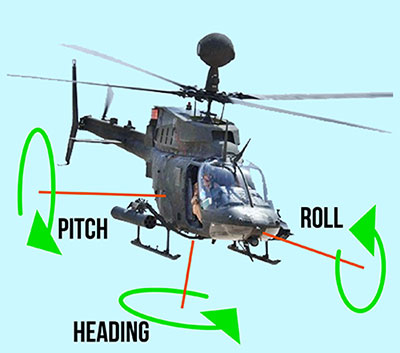
\includegraphics[width=0.30\textwidth]{figures/pitch-roll-heading.jpg}
    \caption{Orientação espacial de uma aeronave: arfagem (\textit{pitch}), rolagem (\textit{roll}) e guinada (\textit{heading}).}
    \label{fig:helicoptero}
\end{figure}

    
\section{Especificação}\label{Sec:EspecifDesemp}
    Os requisitos de desempenho no domínio do tempo adotados para o controle de pitch foram:

\begin{enumerate}
    \item \textit{Overshoot} máximo percentual: $M_{p} \leq 30\%$;
    \item Tempo de acomodação: $t_{2\%} \leq \SI{20}{\s}$; e
    \item Erro nulo em estado estacionário para entradas do tipo degrau.
\end{enumerate}

Os requisitos de desempenho no domínio do tempo adotados para o controle de yaw foram:

\begin{enumerate}
    \item \textit{Overshoot} máximo percentual: $M_{p} \leq 20\%$;
    \item Tempo de acomodação: $t_{2\%} \leq \SI{10}{\s}$; e
    \item Erro nulo em estado estacionário para entradas do tipo degrau.
\end{enumerate}


Tais requisitos introduziram restrições que delimitaram uma região de suposto desempenho satisfatório no plano complexo $s$, e foram consideradas no projeto dos controladores.


\section{algoritmo}\label{Sec:algoritmo}
    O sistema é composto por dois rotores de velocidade variáveis, sendo uma hélice horizontal e outra vertical, acoplado em uma haste com dois graus de liberdade que por sua vez está conectada a uma outra haste com contra-peso.
A planta possui duas variáveis de entrada, que são as tensões de alimentação de cada rotor, fornecidas pela unidade eletrônica, que recebe uma referência de $-2.5$ a $\SI{2.5}{\volt}$ do controlador. Também possui duas variáveis a serem controladas, correspondente aos dois graus de liberdade: ângulo de arfagem e angulo de guinada, sendo sensoreadas, cada uma, por \textit{encoders} incrementais, lidos pela unidade de aquisição de dados e enviados ao controlador \cite{ManualRotor}.

\begin{figure}[H]
    \centering
    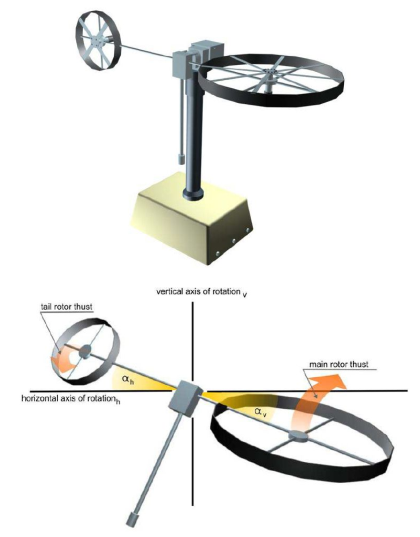
\includegraphics[width=0.30\textwidth]{figures/twin_rotor.PNG}
    \caption{Dispositivo \textit{Twin rotor MIMO System}.}
    \label{fig:TwinRotor}
\end{figure}

No sistema físico está presente a perturbação de fluxos de ar externos e turbulências. Como não-linearidades, tem-se o atraso da aceleração do rotor e de seu empuxo. O torque de arfagem depende de forma não-linear da orientação espacial.

Tem-se como variável controlada o ângulo de arfagem (\textit{pitch angle}), responsável pelo movimento vertical do rotor dianteiro. A tensão aplicada ao rotor é a variável manipulada. O \textit{set-point} ou referência é o ângulo de arfagem desejado, que nessa prática foi expresso em sinais do tipo degrau, senoide e rampa. A variável medida foi o ângulo de arfagem real do rotor (resposta do sistema).

% Para realizar o controlador, optou-se por operar em uma faixa próxima da posição horizontal, a fim de aproximar a planta para um sistema linear.

    
\section{Resultados Experimentais}\label{Sec:resultados}
	
\subsection{\textbf{Teste do Controlador na Planta}}

Simulamos os controladores, até que estivessem com um desempenho satisfatório. Então foram realizados ensaios com uma entrada variável, para realizar a observação de desempenho dos controles com desacoplamento, correspondentes às figuras \ref{fig:ResultadosYaw}, \ref{fig:ResultadosPitch}.
É possível observar que o desempenho foi satisfatório e condizente com os requisitos.

\begin{figure}[H]
    \centering
    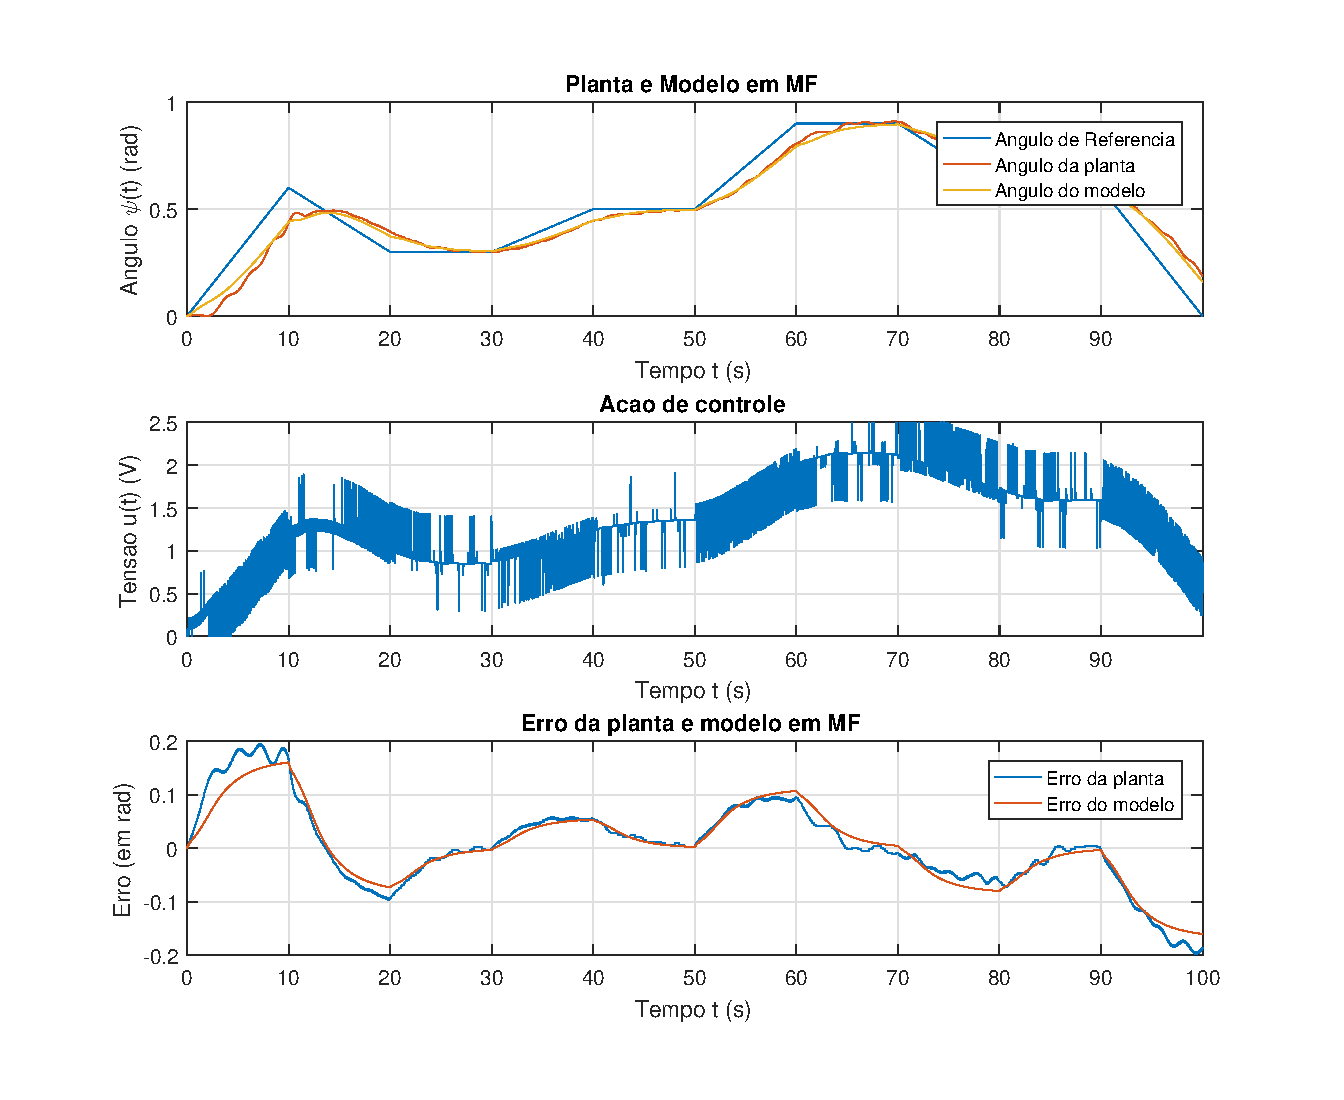
\includegraphics[width=0.5\textwidth]{figures/resultados/valida_pitch.eps}
    \caption{Validação de controle desacoplado de  \textit{pitch}.}
    \label{fig:ResultadosPitch}
\end{figure}

\begin{figure}[H]
    \centering
    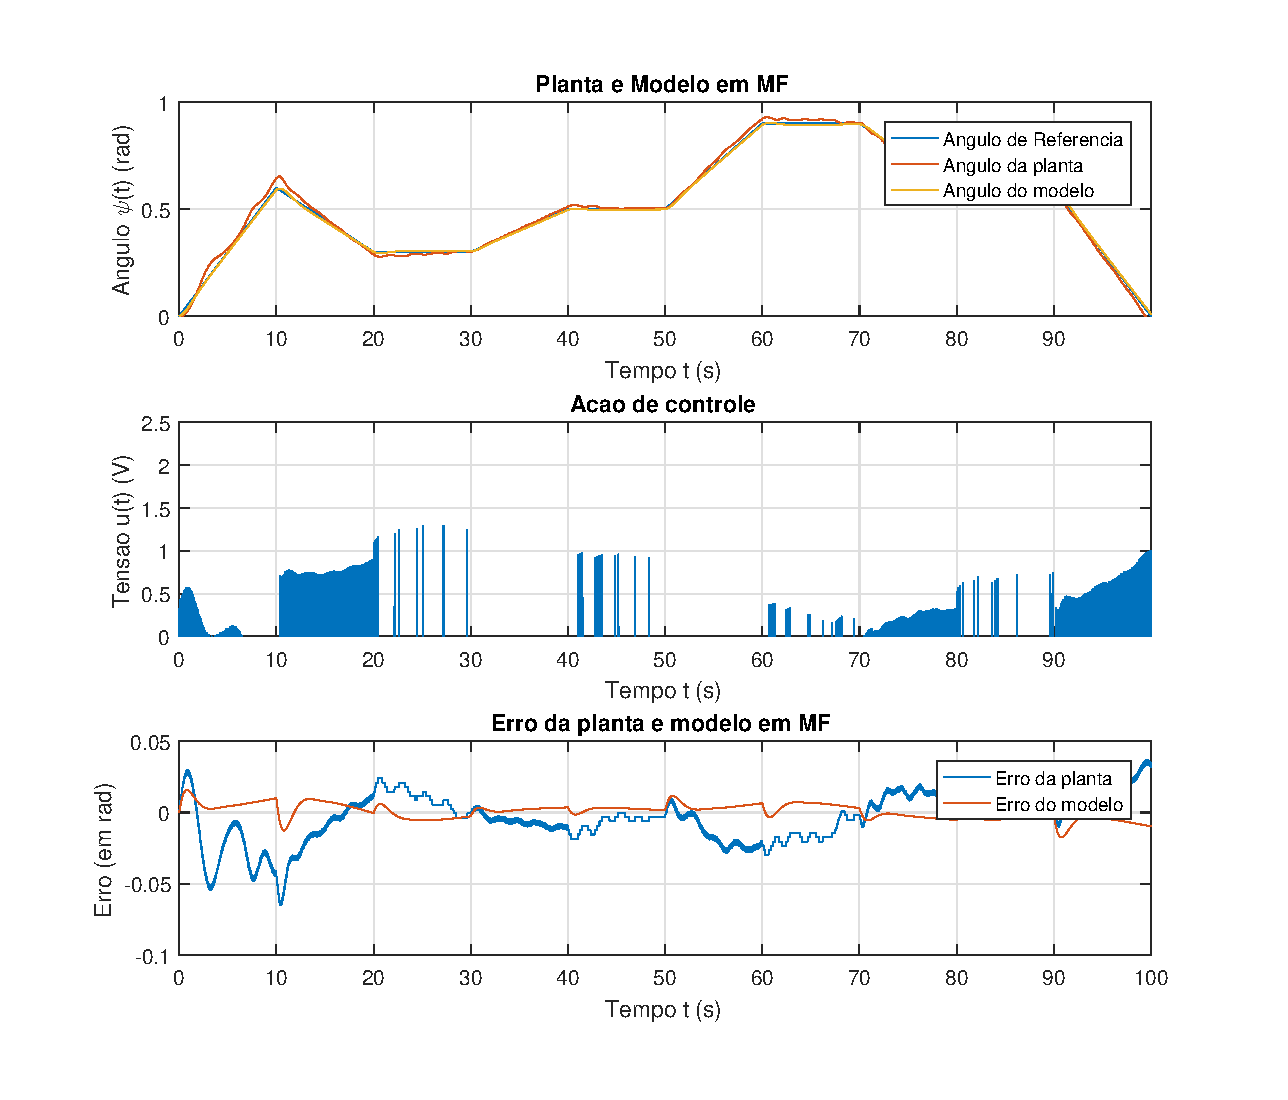
\includegraphics[width=0.5\textwidth]{figures/resultados/valida_yaw.eps}
    \caption{Validação de controle desacoplado de  \textit{yaw}.}
    \label{fig:ResultadosYaw}
\end{figure}


\subsection{\textbf{Análise de Desempenho}}

Para a avaliação de desempenho do sistema em malha fechada para a entrada variável mostrada na Figura \ref{fig:ValidaControladorEntradaVariavel}, foi realizada utilizando-se dois índices de desempenho, a Integral do Erro Quadrático (\textit{ISE - Integral Squared Error}) e a Integral do Erro Absoluto (\textit{IAE - Integral Absolute Error}). Os quais foram calculados por meio das equações \eqref{eq:ISE} e \eqref{eq:IEA}
 \begin{equation}\label{eq:ISE}
     ISE = \int_{0}^{T} e^{2}(t) dt
 \end{equation}
 \begin{equation}\label{eq:IEA}
     IEA = \int_{0}^{T} |e(t)| dt
 \end{equation}

\noindent onde $e$ é o erro, dado pela diferença entre o \textit{set-point} e o ângulo medido e $T$ representa a janela de tempo considerada.
 
Para o \textit{yaw}, obtivemos os seguintes índices:
$$ISE = 2.8430 $$
$$IAE = \SI{450.3624}{} $$
E para o \textit{pitch}, obtivemos:
$$ISE = 507.7020 $$
$$IAE = \SI{5.5331e+03}{} $$


	
\section{Conclusões}\label{Sec:ConsiderFinais}
	Por meio dessa prática, foi possível controlar, com desempenho satisfatório, uma planta do tipo MIMO, utilizando a técnica de desacoplamento, dessa forma possibilitando o controle para yaw e pitch independentemente. 

\bibliography{reference}
\bibliographystyle{apalike}

\end{document}
